\documentclass[LaTeX2e,10pt]{beamer}
\usefonttheme[onlymath]{serif}

\usepackage{xcolor}
\usepackage{graphicx}
\usepackage{psfrag}
\usepackage{epstopdf}
\usepackage{hyperref}
\usepackage{bookmark}
\usepackage{lmodern}

\definecolor{sotonMB}{rgb}{0 0.3594 0.5156} % soton marine blue (7469)
\definecolor{sotonCB}{rgb}{0.1 0.6844 0.7703} % soton cyan blue (3145)
\definecolor{sotonLB}{rgb}{0 0.5938 0.7617} % soton light blue (313)
\definecolor{sotonDG}{rgb}{0.3164 0.3828 0.4336} % soton dark grey (7545)
\definecolor{sotonGR}{rgb}{0.6367 0.5653 0.4180} % soton green (5777)
\definecolor{sotonME}{rgb}{0.7305 0.7305 0.7305} % soton metal (877)
\definecolor{sotonLG}{rgb}{0.6406 0.6797 0.7070} % soton light grey (7543)

\definecolor{sotonyel}{rgb}{.99999 .70196 .00000} % soton yellow
\definecolor{sotonora}{rgb}{.99608 .24314 .07843} % soton orange
\definecolor{sotonred}{rgb}{.94118 .05882 .17255} % soton red
\definecolor{sotonrus}{rgb}{.67059 .07059 .06275} % soton russet
\definecolor{sotonbrn}{rgb}{.54118 .25490 .16863} % soton brown
\definecolor{sotonpnk}{rgb}{.88627 .41176 .62353} % soton pink
\definecolor{sotonppl}{rgb}{.32549 .12157 .26667} % soton purple

\setbeamertemplate{background canvas}[vertical shading][top=sotonMB,bottom=sotonCB]
\setbeamercolor{background canvas}{bg=}
\setbeamercolor{button border}{bg=sotonMB, fg=sotonCB}
\setbeamercolor{button}{bg=sotonMB, fg=DarkRed}

\setbeamercolor{title page}{fg=white}

\setbeamercolor{block title}{fg=sotonMB}
\setbeamercolor{frametitle}{fg=sotonMB}
\setbeamercolor{framesubtitle}{fg=sotonMB}
\setbeamercolor{alerted text}{fg=sotonMB}
\setbeamercolor{normal text}{fg=darkgray}
\setbeamercolor{titlelike}{fg=sotonMB}
\setbeamercolor{author}{fg=darkgray}
\setbeamercolor{date}{fg=darkgray}
\setbeamercolor{item}{fg=darkgray}
\setbeamercolor{caption name}{fg=darkgray}
\setbeamercolor{footline text}{fg=darkgray}

\newcommand{\putlogoUnit}{
\includegraphics[width=3.5cm]{Logos/fee_logo}} % for ISVR
\newcommand{\putlogo}{
\includegraphics[width=3.5cm]{Logos/UOS_White}} % for UoS
\newcommand{\putlogoblue}{
\includegraphics[width=3.5cm]{Logos/UOS_CMYK}}

\newcommand{\footline}{\color{sotonMB}\rule{\textwidth}{1pt}}

\setbeamertemplate{title page}{
	\vskip30pt
	\begin{centering}
		\huge \inserttitle \\ \insertsubtitle 
		\small{
			\vskip20pt
			\insertauthor \\
			\vskip20pt
			\insertdate \\~\\~\\
			
\includegraphics[width=2.5cm]{Logos/esprc_logo}\hspace*{1cm}~%
			
\includegraphics[width=5cm]{Logos/rolls-royce_logo}\hspace*{1cm}~%
			
\includegraphics[width=1cm]{Logos/ngcm_logo} \\
			
			}
	\end{centering}
}

\title{Turbine Blade Design in the Face of Uncertainty}
\author[JK]{Jan Kamenik$^1$, 2nd author$^2$\\~\\ \footnotesize $^1$University of Southampton, UK\\$^2$University of Colorado, USA}
\institute[FEE]{Faculty of Engineering and the Environment\\University of Southampton}
% ----------------------------- END -----------------------------------------------------------------------------------------------------------------

% ---------- FURTHER DEFINITIONS --------------
\setlength{\unitlength}{1cm}
\graphicspath{{./Graphics/}}
% --------------- END -------------------------

\begin{document}

\setbeamertemplate{headline}{
	\vspace{4pt}\hspace{2pt}\putlogoUnit\hfill\putlogo\hspace{3.5mm} % logo on the right
}

\frame{\titlepage}
\addtocounter{framenumber}{-1} % Do not count the title frame!

\setbeamertemplate{headline}{
	\vskip25pt % horizontal line
	\vskip-21pt\hspace{2pt}\hfill\putlogoblue\hspace{3.5mm} % logo on the right
}

\setbeamertemplate{footline}{
	\vskip-10pt\footline\\ % horizontal line
	\vskip2pt
	\makebox[123mm]{\hspace{7.5mm}
	\insertshorttitle
	\hfill \insertframenumber/\inserttotalframenumber}
	\vskip4pt
}

\setbeamertemplate{background}
{
\includegraphics[width=\paperwidth,height=\paperheight]{background.pdf}}

%\begin{frame}
%	\frametitle{Table of Contents}
%	\tableofcontents[currentsection]
%\end{frame}

\section{Introduction}

\begin{frame}{Speaker Background}
\begin{enumerate}
	\item 1
\end{enumerate}

Full project title: ...
\end{frame}

\begin{frame}{Introduction}
	\vskip7pt
\begin{figure}[h!]
	\centering
	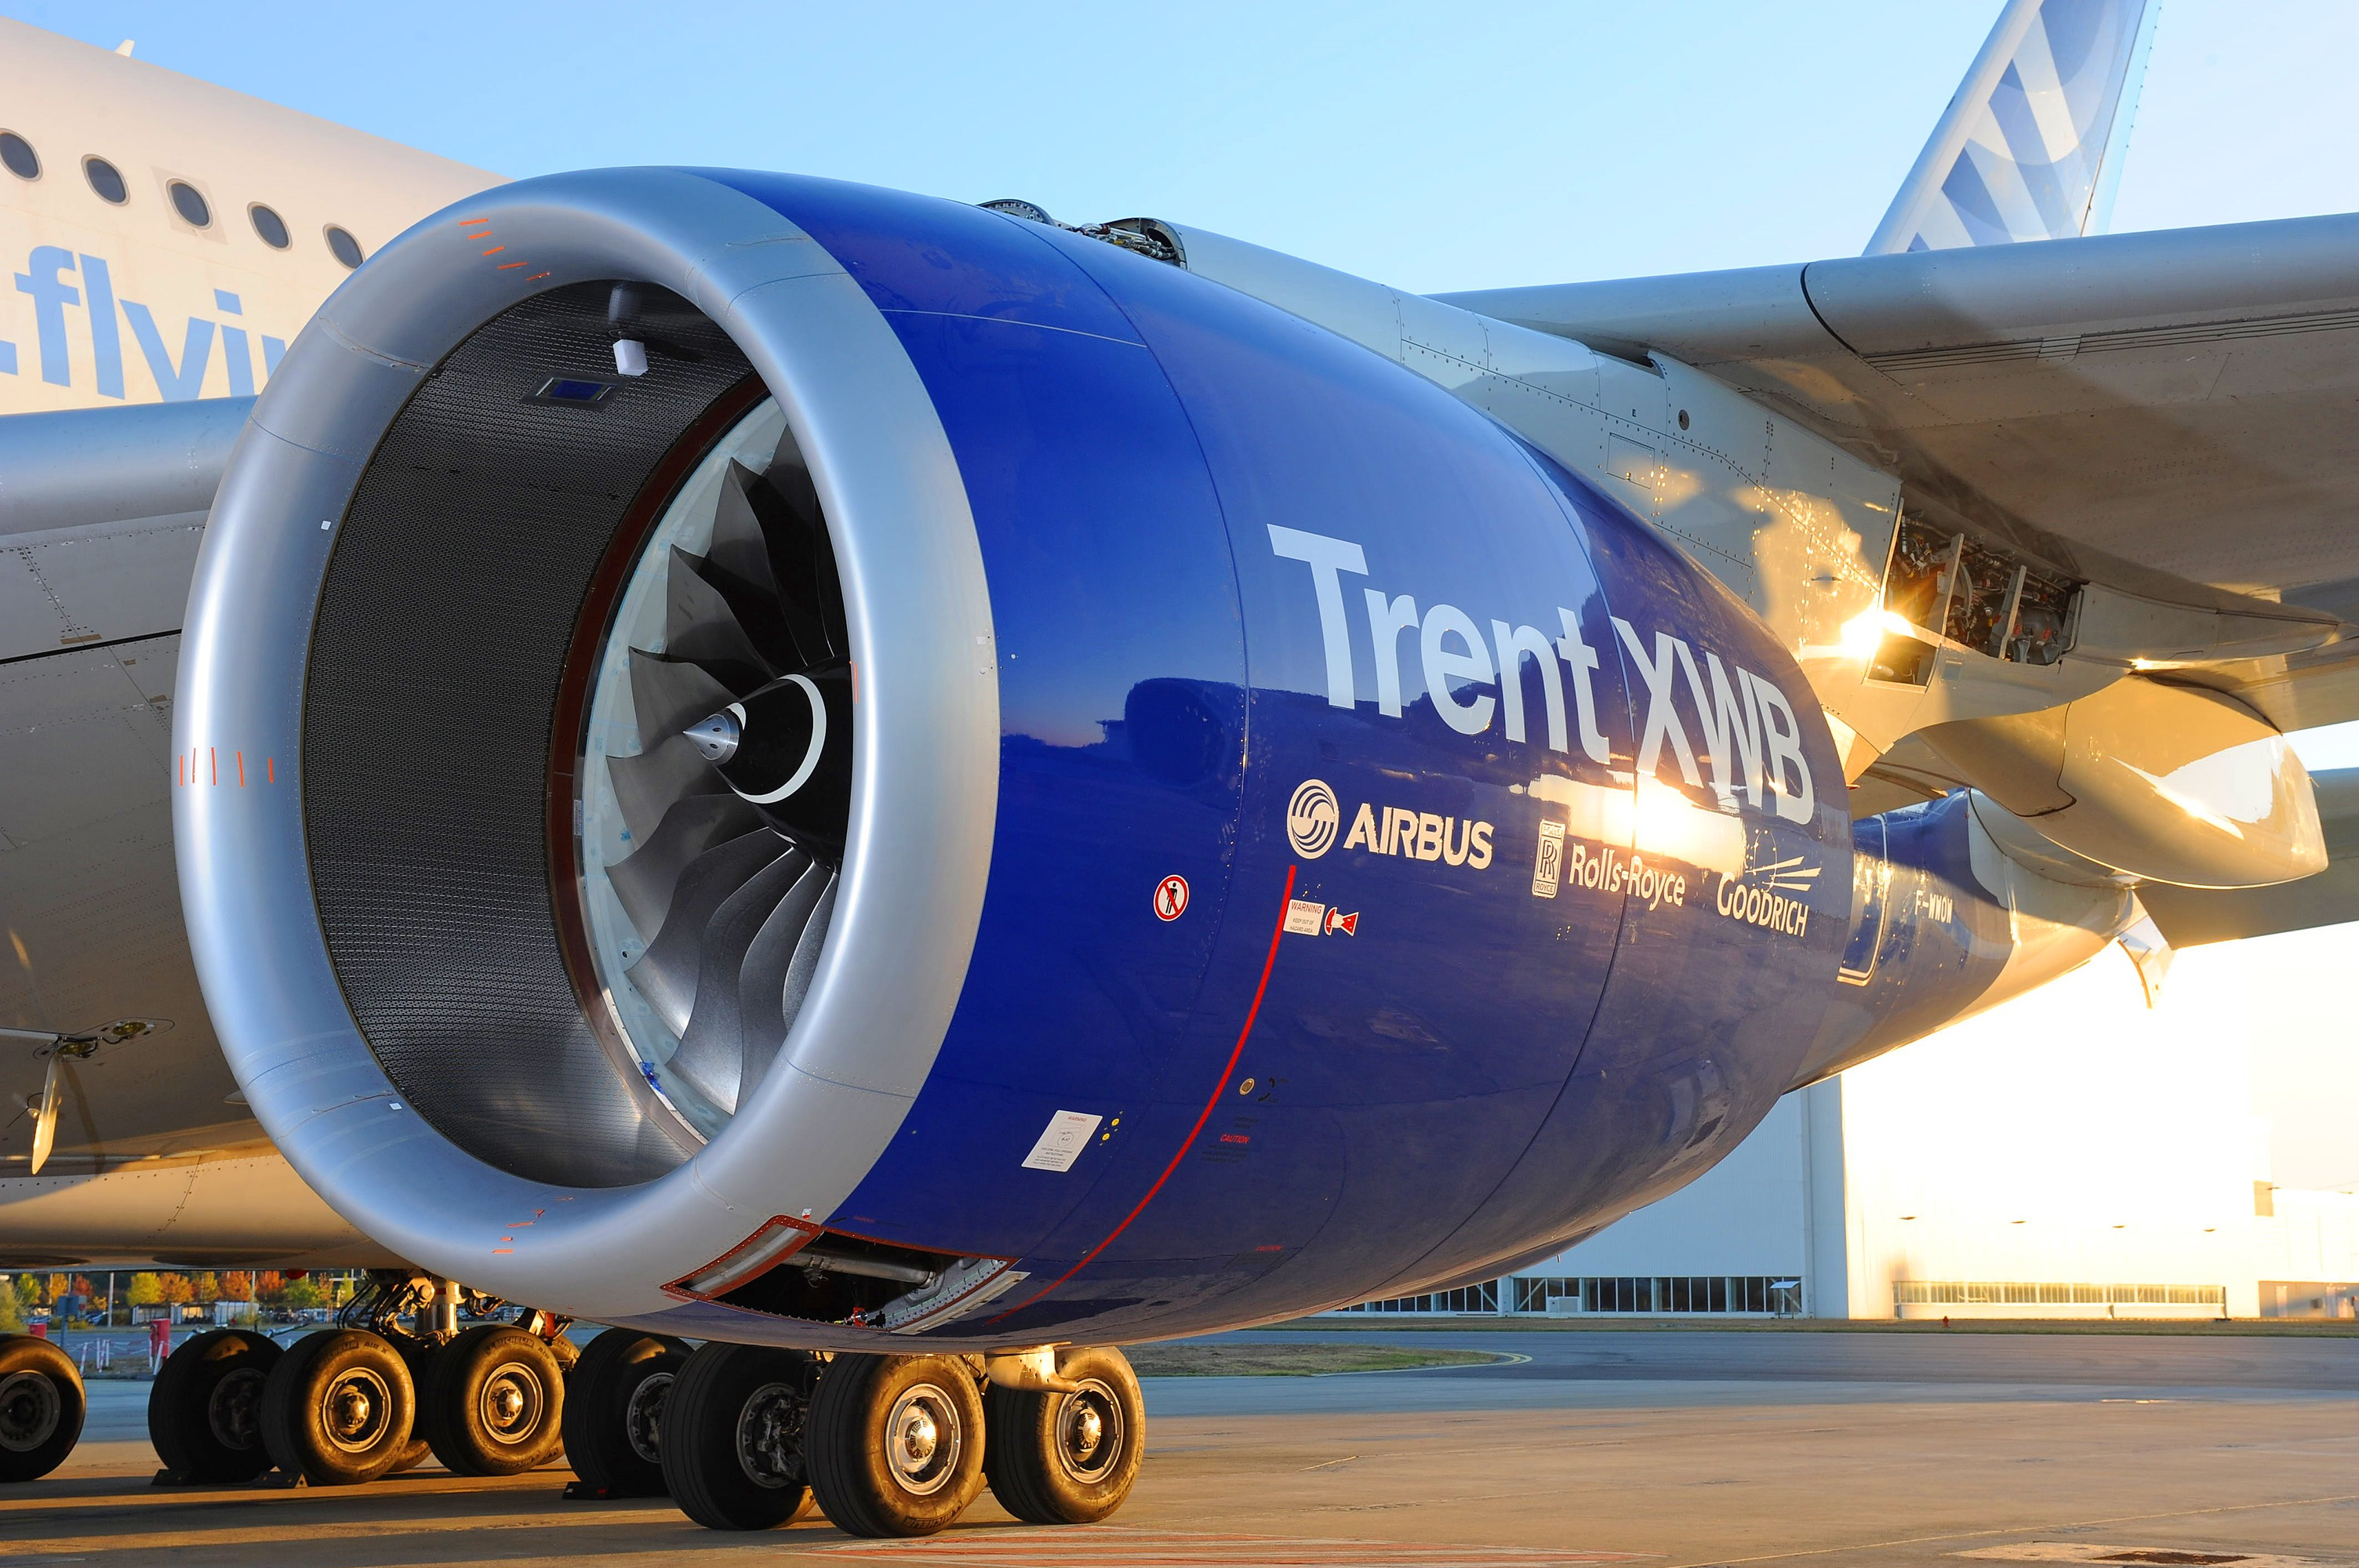
\includegraphics[width=0.9\linewidth]{Graphics/A350_XWB.jpg}
	\caption{Trent XWB turbofan}
	\label{fig:xwb}
\end{figure}
\end{frame}

\begin{frame}{Introduction}
	\vskip7pt
	\begin{figure}[h!]
		\centering
		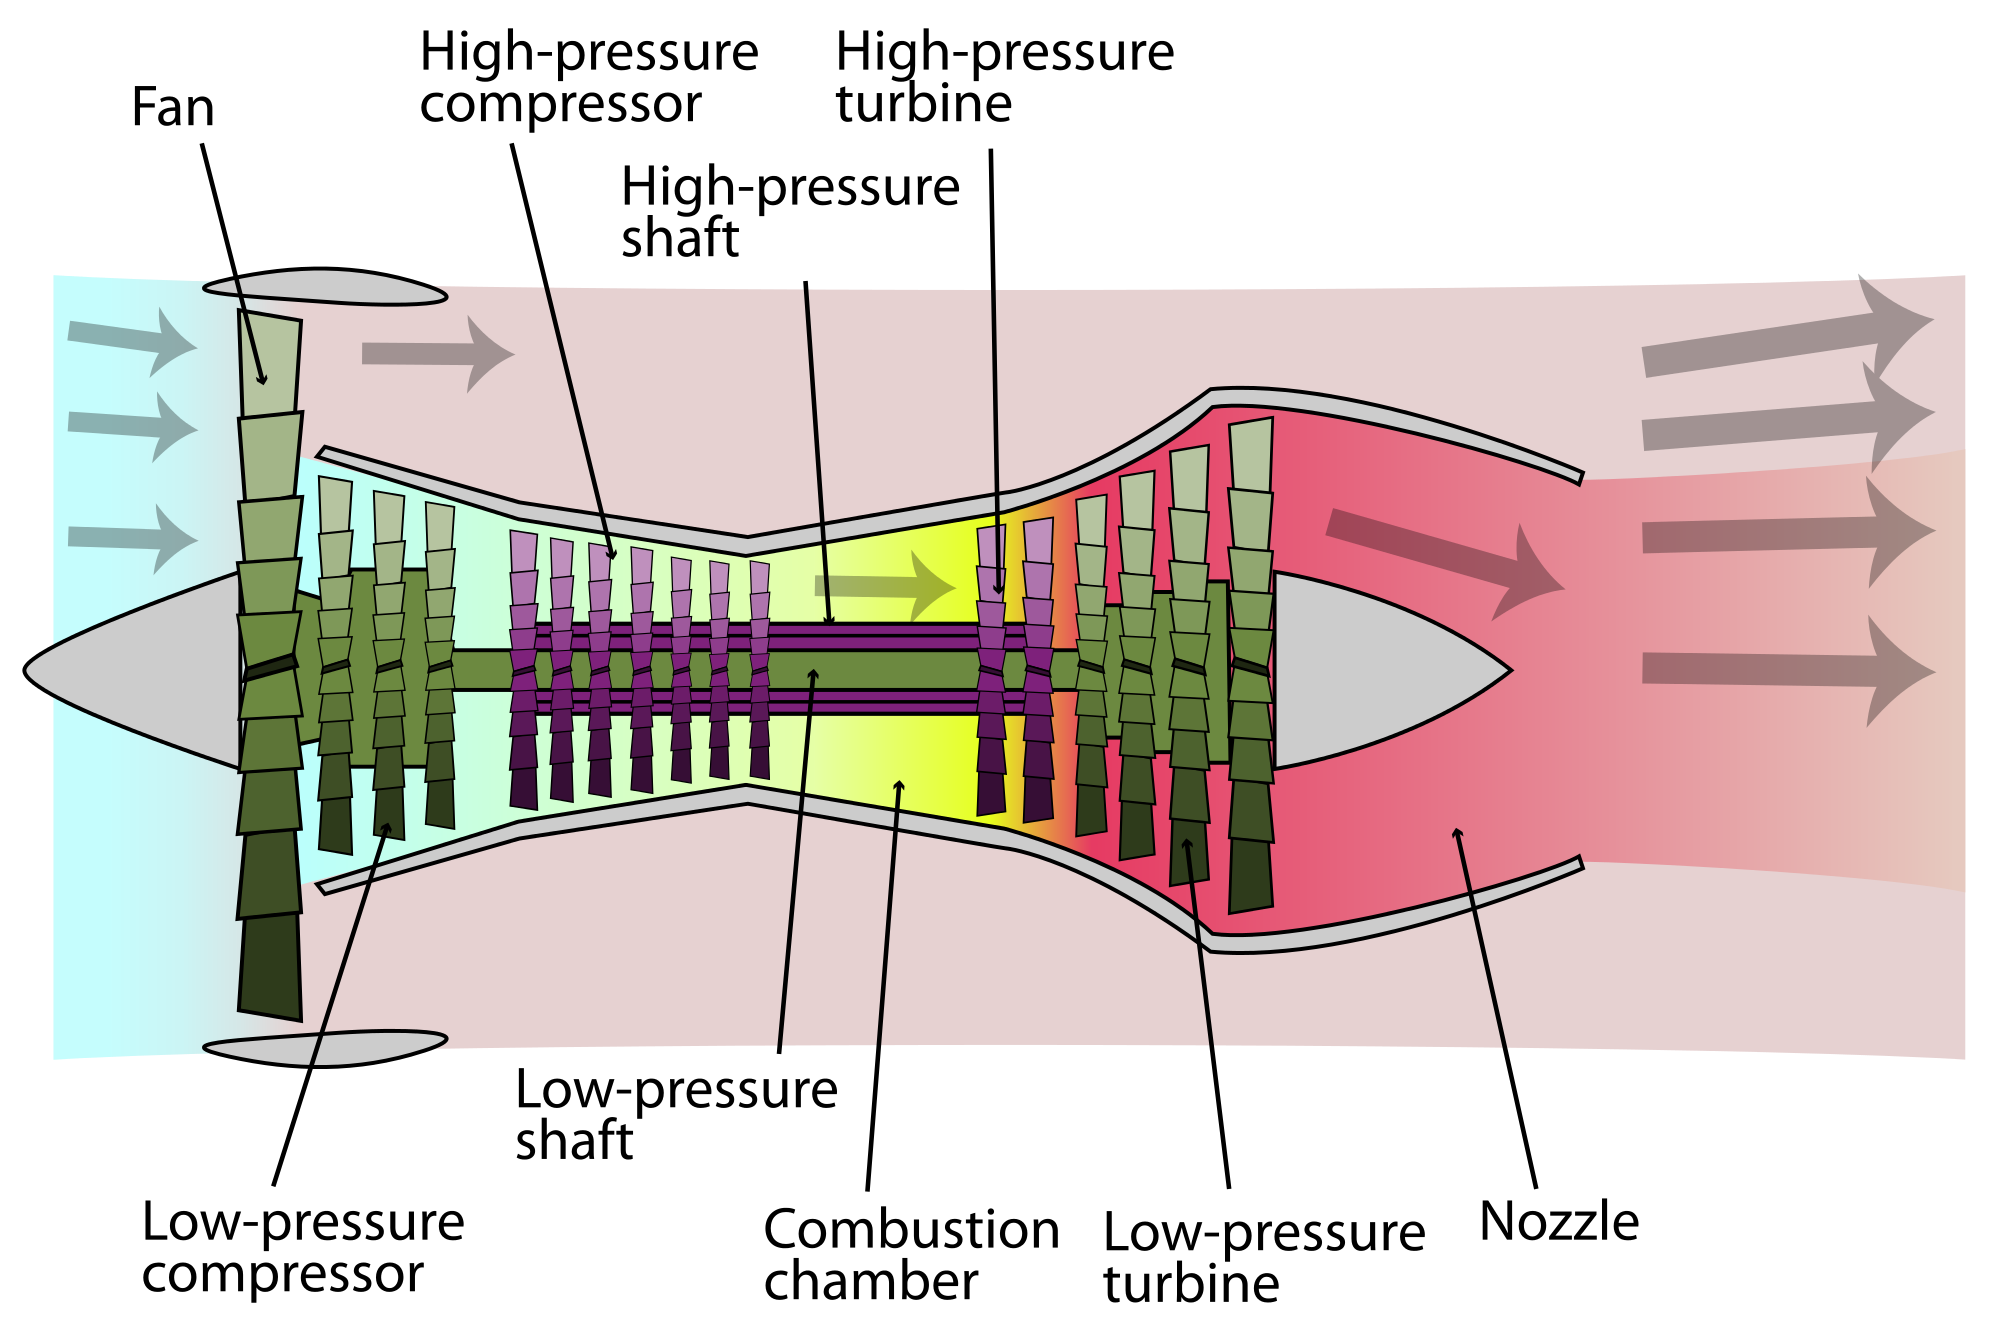
\includegraphics[width=0.9\linewidth]{Graphics/2000px-Turbofan_operation.png}
		\caption{Major components of turbofans}
		\label{fig:turbofan}
	\end{figure}
\end{frame}

\section{Main content}

\begin{frame}{Turbine Blades}{This is a subtitle example}
	\begin{enumerate} [<+->]
		\item item 1
		\item item 2
	\end{enumerate}
\end{frame}

\section{Conclusions}

\begin{frame}{Conclusions}
	Some conclusions
\end{frame}

\end{document}